\chapter{Introduction}


\section{Cosmology and the cosmic dawn}

\subsection{Modern cosmology and the history of the universe}

Much like particle physics, cosmology today finds itself in the enviable yet frustrating position of having a broadly supported picture of the universe with only the most challenging and fundamental questions unanswered. Many intersecting lines of evidence point to a universe which was hot, dense, homogenous, and rapidly expanding 13.8 billion years ago. It eventually cooled enough for bound objects to form and is now expanding at an accelerating rate. Studies of the cosmic microwave background (CMB), high-z supernovae, distant galaxies, primordial element abundances, the matter power spectrum, and other observables all converge on this model. It is largely, however, a poorly understood and entirely unexpected \textit{dark} universe, whose total energy budget is dominated by constituents whose gravitational properties are well understood, but whose fundamental nature remains mysterious. 

The simplest (i.e., \textit{vanilla}) model which agrees with all available data is parameterized by the energy densities of baryons ($\Omega_bh^2=0.0222\pm0.0002$), cold dark matter  ($\Omega_ch^2=0.119\pm0.002$), and vacuum energy ($\Omega_\Lambda=1-\Omega_b-\Omega_c$), as well as the amplitude ($10^{9}A_se^{-2\tau}=1.881\pm0.014$) and spectral index ($n_s=0.9652\pm0.0062$) of the primordial power spectrum, and the optical depth to reionization ($\tau=0.078\pm0.019$). 
The energy densities are given as the present densities of these constituents relative to the present critical density $\rho_c=3H_0^2/8\pi G$, where the present expansion rate is $(70\pm3$)\,km/s/Mpc
\footnote{I've taken the uncertainty on $H_0$ to be the spread between the CMB measurement of $67.74\pm0.46$ km/s/Mpc \citep{planck16} and the local measurement of $73.2\pm1.7$ \citep{reiss16}.}. 
On scales larger than hundreds of Mpc, our universe is flat, deviating from Euclidian geometry only due to a homogenous and isotropic expansion, with a measured curvature density consistent with zero of $\Omega_K=0.008\pm0.004$. 
Further, the equation of state of dark energy is constrained to be $w=-1.02\pm0.08$, consistent with -1, and thus, with a true cosmological constant or a uniform vacuum energy. These measurements represent the best combined constraints reported by \citet{planck16}, and have been made possible by the avalanche of data on the CMB, weak lensing statistics, baryon acoustic oscillations, and type 1a supernova surveys collected in recent years. 

In this framework, the history of the universe is fairly well established. Nuclear reactions in the first few minutes of the universe created hydrogen, helium, and trace amounts of deuterium and lithium, and astronomers have verified these predictions of primordial abundances to high precision \citep{bbn}. After 370,000 years of expansion and cooling, the photon mean free path increased to larger than the Hubble radius, and protons and electrons combined to form atoms. These relic photons fill the universe and are known as the CMB; their non-uniformities (i.e., anisotropies) evidence $\sim10^{-5}$ density and temperature fluctuations at the epoch of recombination. After the release of the CMB, but before before the first stars formed, these slight fluctuations underwent gravitational collapse during a period known as the dark ages ($20\lesssim z\lesssim 1100$). After a few hundred million years, sufficient temperatures and pressures were reached in these collapsing halos to stave off further collapse, resulting in the first luminous sources in a period known as the cosmic dawn. These first stars (termed population III) formed from pristine gas, uncontaminated by metals\footnote{In astronomy nomenclature, all atoms heavier than Helium are known as \textit{metals}.} formed in the cores of later generations of stars or in supernovae. Without the fine structure lines of these metals, these stars failed to collapse and cool as efficiently as modern stars, resulting in hot, massive stars whose ultraviolet emission eventually ionized the entire intergalactic medium. This is the epoch of reionization ($6\lesssim z\lesssim12$).

Though this basic sequence of events is well understood, many questions remain. How massive were this first generation of stars? How bright? How numerous? What were the relative contributions of stars, black hole binaries, and quasars to the ionizing photon budget? When exactly did these first stars form and how long did it take? How much did the next generation of stars (population II) contribute to the reionizing process? Simple N-body simulations can model the gravitational collapse of the cosmic web and dark matter halos, but empirical feedback and star formation models are needed to understand the the baryonic\footnote{In astronomy nomenclature, all particles other than dark matter are termed \textit{baryons}, whereas in particle physics, a \textit{baryon} refers specifically to a bound state of three quarks such as a proton or a neutron.} processes. It is no wonder progress has been slow: these stars and galaxies are by definition the farthest and faintest ones that one can ever hope to observe. Understanding their formation, before any stars even shone at all, is even more of a challenge to observers. 

This thesis presents experimental work in the field of 21\,cm cosmology, a promising avenue to circumvent the catch-22 of how to observe galaxies before they began to emit light. The idea, which I overview in Sec. \ref{sec:intro21cmsection}, is to study \textit{not} the galaxies themselves, but the diffuse gas between them. In particular, we seek to measure the faint low frequency radio emission from the neutral hydrogen between galaxies in order to map out the ionized bubbles growing around galaxies over cosmic time, and eventually the global matter distribution of the universe. 


\subsection{Reaching towards the cosmic dawn}

For all the questions about the astrophysics of reionization and the lack of direct observations, a number of indirect constraints establish a rough picture of the EOR and bound its beginning and end. 

% Ly-alpha forest
The evolution of the Lyman alpha forest in quasar spectra into a ``trough'' of complete absorption (Gunn-Peterson trough) blue-ward of Ly$\alpha$ in $z\sim6$ quasars provide perhaps the clearest evidence of the evolving ionized fraction of the IGM. Quasars are an observational category of active galaxies whose smooth spectrum jets are oriented and Doppler-boosted along our line of sight, appearing very bright. At redshifts $1<z<3$ the band between Lyman continuum and Lyman-$\alpha$ becomes increasingly crowded with absorption lines, indicating that these quasar beams have traversed more and more neutral hydrogen clouds at intermediate redshifts. Between $3<z<5$, these lines become so crowded, that there is no apparent continuum level, and at higher redshifts close to the end of reionization at $z\sim6$, there are enough neutral hydrogen atoms left in the IGM that all emission in this band is absorbed. A caveat is that the Lyman alpha line saturates at even very small neutral fractions of $\gtrsim 10^{-5}$ \citep{FurlanettoReview}, so the appearance of a Gunn-Peterson trough is evidence only of the tail end of reionization. The mid point and indeed the whole reionization history is unconstrained by these observations.

\begin{figure}
	\centering
	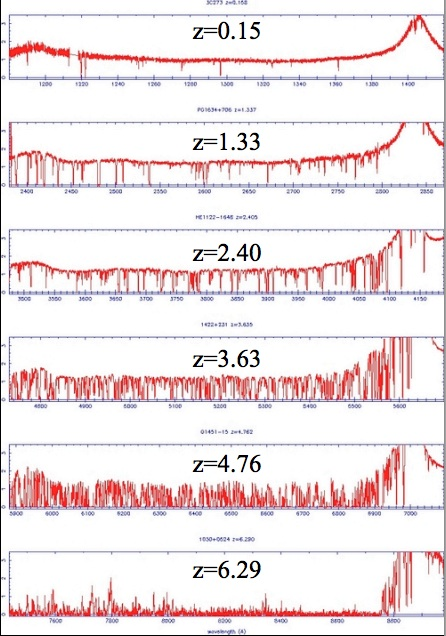
\includegraphics[width=3in]{chap0_intro/lymanalpha_diffz.jpg}
	\caption[Quasar spectra from low to high redshift, showing the transformation of the Ly-$\alpha$ forest into the Gunn-Peterson trough.]{Quasar spectra from low to high redshift, showing the transformation of the Ly-$\alpha$ forest into the Gunn-Peterson trough. Figure credit to Ross McLure.}
	\label{fig:lya}
\end{figure}

% CMB optical depth measurements
An orthogonal constraint on the redshift of reionization derives from the measurement of the Thomson scattering optical depth $\tau$ between us and recombination. Scattering of CMB photons off free electrons tends to smear out the temperature anisotropies, damping the power on all angular scales scales as $e^{-2\tau}$. However there are no free electrons in the intergalactic medium prior to reionization, so such scattering does not occur until after that epoch.  Assuming reionization occurred instantaneously at $z_\text{re}$, the thompson scattering optical depth is 
\begin{equation}
\label{eqn:opticaldepthcmb}
	\tau=\int n_e\sigma_t ds=\sigma_t c\int_0^{z_{re}}\frac{dz}{H(z)(1+z)}\frac{\Omega_M(1+z)^3\rho_c}{m_p}
\end{equation}
where $n_e$ is the number density of free electrons, $\sigma_t$ is the Thomson scattering cross section, $\rho_c=3H_0^2/8\pi G$ is the present critical density of the universe, and $m_p$ is the proton mass. Recent constraints by \citep{plancktau16} give  $\tau=0.06\pm0.01$, depending on the priors used and which other constraints are included, implying a reionization redshift of $z_{re}=9\pm1$ using Eqn. \ref{eqn:opticaldepthcmb}.

This is far from the end of the story, though. Reionization did not occur instantaneously, and the detailed evolution of the ionized fraction over redshift affects this calculation. In fact \citet{bowman2010} set a lower limit of $\Delta z>0.06$ (95\%) on the duration of reionization based on lack of an abrupt step in the low frequency radio spectrum. This indicates the lack of such a step in the 21\,cm global signal over redshift. 

A complication is that the optical depth is somewhat degenerate with the amplitude $A$ of the primordial power spectrum on all but the largest angular scales. There \textit{is} a large angular scale peak in the CMB's E model polarization power spectrum due to the proximity of ionized bubbles to us, but both this large angular scale signature is strongly limited by cosmic variance uncertainties. Constraints on the midpoint and duration of reionization would go a long way toward pinning down the astrophysics of the EOR \citep{liu15a}.

% deep galaxy surveys (photometry) (Hubble and JWST)
A further indirect constraint on the EOR derives from deep galaxy surveys and cluster lensing surveys, which are finding tens of EOR galaxies at $6<z<10$ \citep{Bouwens2011,Illingworth2013,Dunlop2013}, probing down to $M_{AB}\sim-17$. See the review by \citet{madau14review} Note that these high-$z$ galaxies are properly referred to as \textit{candidates} though, as their redshifts are estimated photometrically given that they are generally too faint for spectroscopy. Such observations directly probe the UV luminosity function, which, after assuming an escape fraction and faint end slope, constrains the reionization history. \citet{RobertsonReionization2015} calculate the implied optical depth to the CMB and find reasonable agreement with the latest $\tau$ results from Planck analyses, in contrast to earlier Planck \citep{Robertson2013} and WMAP \citep{hinshaw_et_al_2012} results. Still, the uncertainties are large and the James Webb Space Telescope (JWST) will be needed to probe down to the $M_{AB}\sim-13$ galaxies thought to generate the bulk of the ionizing photons.

Cross correlation experiments comparing these EOR galaxies with 21\,cm observations should provide an important cross check on these results, though the mismatched resolutions of radio and optical/infrared telescopes pose a problem. The full Hubble deep field with its hundreds of high redshift galaxies fits easily inside a single $\sim3'$ resolution element of typical radio survey telescope such as the Murchison Widefield Array (MWA). One possible solution is to compare the galaxies found in 21\,cm bright spots with those found in 21\,cm dark spots, as the latter should be more characteristic of the ionizing population \citep{beardsley15}. Ly-$\alpha$ intensity mapping, as opposed to studies of individual high-$z$ galaxies, is another possible route to probing the EOR source population, and in Ch. \ref{chap:xcor} I present the first limits on the 21\,cm--Ly$\alpha$ broad band cross spectrum.

Other probes are also beginning to bring the EOR into focus, but many require significant assumptions or empirical fitting to relate their predictions to the EOR. Stellar archeology is the study of the oldest, most metal poor (Population II) stars in our own galaxy. These stars formed from gas enriched by only a few supernovae events, and their chemical abundances constrain the properties of the supernovae of first generation stars (Population III), which will eventually allow us to constrain the properties of these first stars \citep{Frebel2015}. Further, N-body simulations can shed light on the mass and luminosity function of the first galaxies and reionization, albeit after incorporating empirically motivated models of complex astrophysical feedback \citep{Bauer2015,Vogelsberger2014} . Lastly, semi-numerical EOR simulations like 21cmFAST \citep{21cmfast} parameterize the EOR with a small number of astrophysical parameters, simplifying the extraction of astrophysical constraints from 21\,cm observations \citep{PoberNextGen,PoberPAPER64Heating}. 

For all the community has pieced together about the epoch of reionization, it is worth emphasizing that many questions remain unanswered. Which galaxies generated the bulk of ionizing photons, and what fraction of their photons reached the IGM? What were the masses and luminosities of Population III stars, when did they form, and what did their supernovae look like? What role did pre-reionization sources like black hole binaries and AGN feedback play in heating the intergalactic medium? And eventually, can we understand and model all this \textit{gastrophysics} to get at the primordial matter power spectrum of the universe, and from there, constrain the underlying cosmology?

\section{Theory of 21cm tomography}
\label{sec:intro21cmsection}

\subsection{Radio emission from neutral hydrogen}

A standard result of quantum mechanics \citep[e.g.,][]{griffithsqm} is that, to first order, the energy levels of the Hydrogen atom are $E_n=(-13.6\,\text{eV})/n^2<0$, where $n=1,2,3,...$. Each state is a solution to the Schrodinger equation describing an electron bound to a proton, neglecting their finite sizes, intrinsic spins, and relativistic effects. At thermal equilibrium, statistical mechanics predicts that the relative fraction of atoms in the $n$'th state is given by the Boltzmann factor $e^{-E_n/kT}$, so that typically only low integer states are populated, and transitions between them release the energy differences as ultraviolet, optical, or near infrared photons. 

At higher order, relativistic effects shift the energy levels, and the coupling of the electron's spin and orbital angular momentum split each $n$ state into several $\ell$ states. These effects produce the \textit{fine structure} in the hydrogen spectrum, though as the ground state has no orbital angular momentum, it is not split at this order. 

\begin{figure}
	\centering
	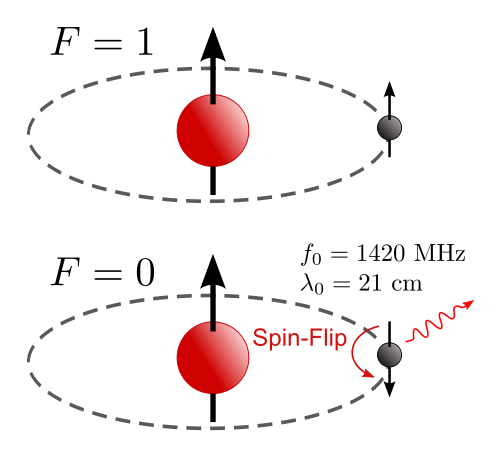
\includegraphics[width=4in]{chap0_intro/500px-Hydrogen-SpinFlip.png}
	\caption[Diagram of the two Hydrogen ground states resulting from hyperfine splitting.]{Typical visualization of the two Hydrogen ground states resulting from the hyperfine splitting \citep{HydrogenSpinFlipGraphic}, where $F$ is the total angular momentum of the system, and the transition between the two states results in emission or absorption of a 21\,cm photon.}
	\label{fig:HydrogenSpinFlipGraphic}
\end{figure}

At the next higher order, the coupling of the proton and electron spins splits all states into those where these spins are parallel and those where they are antiparallel, as in Fig. \ref{fig:HydrogenSpinFlipGraphic}. The energy difference is much smaller than the differences between the $n=1,2,3,...$ states, and corresponds to emission or absorption of a low frequency radio photon with wavelength 21\,cm. In the upper (lower) state the spins are parallel (anti-parallel). Note that this disagrees with classical intuition, as when the spins are parallel, the magnetic dipole moments are antiparallel, and just as two antialigned magnets tend to attract, this state \textit{should} have \textit{lower} energy. 

In response, is often remarked simply that quantum mechanics sometimes makes counterintuitive predictions, though \citet{griffiths82} argues that there is a more intuitive way to understand the situation. He observes that Fig. \ref{fig:HydrogenSpinFlipGraphic} misleadingly suggests that the in the $n=0$ state, the electron is displaced from the proton, when in fact its spherical wavefunction encompasses it. It is thus more correct to picture their magnetic moments as due to tiny current loops centered around the nucleus in the plane perpendicular to their spins. If both spins are aligned, then the current loops flow in opposite directions, and thus repel just like parallel wires with opposite currents, explaining which this is the higher energy state.

Lastly, note that in the upper state when the spins point in the same direction, the quantization of $z$ angular momentum makes this actually a spin triplet state, so there are three upper states and one lower state.

\subsection{21cm emission from the Dark Ages and Epoch of Reionization}

In this section I go through a straightforward theoretical calculation of the observed 21\,cm brightness temperature of a neutral cloud in the intergalactic medium (IGM) during the Epoch of Reionization (EOR). I mainly follow \citet{PritchardLoebReview} but fill in many details and background information where helpful. 

\subsubsection{Microscopic radiative transfer using Einstein A and B coefficients}

The Hydrogen atom is not a simple quantum mechanical system; even less so taking into account fine and hyperfine structure. Fortunately in the cool, dilute intergalactic medium, the problem simplifies greatly. Essentially all hydrogen atoms are in the ground state at temperatures  $T<<10\text{eV}/k_B\sim10^5$K, which is always the case before the EOR when gas temperatures are $10-100$\,K, and after the EOR when they are $100-1000$\,K \citep{FurlanettoReview}. Thus only the hyperfine ground states are allowed, and we may regard such atoms at two level systems with an energy spacing of $\Delta E=hc/\lambda\approx6\mu$\,eV, where $\lambda=21$\,cm, and there is a three-fold degeneracy of the upper state. The four states are roughly equally populated as $T>>\Delta E/k_B =0.06$K, giving number densities of excited and ground state atoms which we write as $n_2=\frac{3}{4}n_H$ and $n_1=\frac{1}{4}n_H$, where $n_H$ is the overall density of hydrogen atoms. Lastly, note that the spontaneous emission lifetime of the upper excited state is roughly $10^7$\,years.

Before considering radiative transfer through the universe of 21\,cm emission from a hydrogen cloud at high redshift, we first comment on the different parts of this non-thermodynamic equilibrium problem, and present the Einstein A and B coefficients we will use to treat them. The three temperatures in this problem are: (1) the hydrogen gas temperature, which encodes the root mean square velocities of the particles; (2), the spin temperature, defined as the temperature of an ensemble of two level atoms having the same ratio of excited to ground state atoms as our system; and (3) the temperature of the cosmic microwave background, a blackbody radiation field which backlights our neutral hydrogen clouds during the EOR. 

Our task is to calculate the emergent intensity through an HI cloud with optical depth $\tau$ backlit by the CMB. From standard radiative transfer theory, the answer is $I_\nu=I_0e^{-\tau}+S_\nu(1-e^{-\tau})$, however because our three temperatures are not the same, the source function 
\begin{equation}
S_\nu\equiv j_\nu/\alpha_\nu	
\end{equation}
does not in general equal a Planck (i.e., blackbody) function\footnote{The Planck function is given by $B_\nu(T)\propto\nu^3/(e^{h\nu/kT}-1)$} and we thus require a microscopic description of the radiation field using the Einstein A and B coefficients.

Consider again our two level atom with number densities $n_2$ and $n_1$ in the excited and ground states, respectively. The Einstein coefficients are defined by:
\begin{eqnarray}
\text{\# spontaneous emissions per volume per time}&=&An_2 \nonumber\\
\text{\# stimulated emissions per volume per time}&=&B_{21}n_2u_\nu \nonumber\\
\text{\# absorptions per volume per time}&=&B_{12}n_1u_\nu 
\end{eqnarray}
where $u_\nu$ is the energy/(volume $\cdot$ frequency) of the radiation field. Note that $A$ has units of $\text{s}^{-1}$, and the $B$'s have units of time$^{-1}$[energy/(volume $\cdot$ frequency)]$^{-1}$. We can construct the unit of energy density per frequency as $h\nu/(c/\nu)^3/\nu$, thus on purely dimensional grounds we expect $A\approx B (h\nu^3/c^3)$. The exact relation from atomic physics is $A=B_{12}8\pi h \nu^3/c^3$. Einstein showed that $g_1B_{12}=g_2B_{21}$ (where in our case $g_1=1$, $g_2=3$) regardless of whether the atoms are in thermal equilibrium with the radiation field.

Before calculating the radiation source function, let us look at the radiative transfer equation to understand how to treat stimulated emission,
\begin{equation}
\frac{dI_\nu}{ds}=j_\nu-\alpha_\nu I_\nu
\end{equation}
where $I_\nu$ is the specific intensity, with units of energy/(area $\cdot$ solid angle $\cdot$ frequency $\cdot$ time), and the absorption coefficient $\alpha_\nu$ has units of length$^{-1}$. Note that the emission coefficient $j_\nu$ thus has units of energy/(volume $\cdot$ solid angle $\cdot$ frequency $\cdot$ time). As the stimulated emission rate is proportional to the radiation density it makes sense to think of it contributing \textit{negatively} to the absorption coefficient, in which case the emission coefficient is due solely to spontaneous emission. We introduce a line shape $\phi(\nu-\nu_0)$ where $\nu_0=1420$\,MHz=c/(21\,cm), and integrate $j_\nu$ over the spectral line to find the energy emitted per volume per time per solid angle:
\begin{equation}
\int j_\nu d\nu=\int\frac{1}{4\pi}h\nu\phi(\nu-\nu_0) n_2 Ad\nu
\end{equation}
which proves that
%If we introduce a line shape $\phi(\nu-\nu_0)$ with $\int\phi(\nu-\nu_0)d\nu=1$, where $\nu_0$ is the center frequency of the spectral line, then we have:
\begin{equation}
j_\nu=\frac{h\nu_0 n_2A\phi(\nu-\nu_0)}{4\pi}
\end{equation}

Now consider a beam with intensity $I_\nu$ passing through the atoms. The energy density in the beam is $u_\nu=I_\nu/c$, so the energy absorbed from the beam per volume per time is $\int d\nu\int\alpha_\nu I_\nu$, which can also be expressed as $\int d\nu h\nu_0\phi(\nu-\nu_0)(n_1B_{12}-n_2B_{21})I_\nu/c$, which gives:
\begin{equation}
\alpha_\nu=\frac{h\nu_0\phi(\nu-\nu_0)(n_1B_{12}-n_2B_{21})}{c}
\end{equation}

Then the source function, defined above, is
\begin{equation}
S_\nu=\frac{c}{4\pi}\frac{ n_2A}{n_1B_{12}-n_2B_{21}}
\end{equation}
which is valid even if the atoms are not in thermodynamic equilibrium with the radiation field. 

\subsubsection{Brightness temperature of an HI cloud in the EOR}

Now let us put the pieces of this calculation together and relate them to the observed emergent intensity of the CMB shining through an HI cloud during the EOR. As above, considering a radiation field with intensity $I_0$ behind a cloud of hydrogen with optical depth $\tau$, the emergent intensity is $I_\nu=I_0e^{-\tau}+S_\nu(1-e^{-\tau})$. Cosmological redshift reduces the observed energy flux by $(1+z)$, and then reformulating the equation in terms of brightness temperatures and assuming $\tau<<1$ (because this is a very weak transition) gives
\begin{equation}
\delta T=\frac{T_s-T_\gamma(z)}{1+z} (1-X_i)\tau
\end{equation}
where the spin temperature $T_s$ is the brightness temperature of 21\,cm radiation from the gas\footnote{We can prove that the spin temperature equals the brightness temperature of the gas noting first that $S_\nu=j_\nu/\alpha_\nu\propto A n_2/(n_1B_{12}-n_2B_{21})\propto\nu^3n_2/(3n_1-n_2)$, using $A\propto\nu^3B$. The spin temperature $T_s$ is defined by $n_2/n_1\equiv3e^{-h\nu/k_B T_s}$, where $n_2/n_1\approx3(1-h\nu/k_BT_s)$ for $T_s>>h\nu_0/k_B= 0.0681$\,K. Putting these together gives $S_\nu\propto \nu^2 T_s$, which is the Rayleigh-Jeans relation with the spin temperature instead of the typical gas temperature}, and $X_i$ is the gas ionized fraction. Now we just need the optical depth through the cloud with size $ds$.

\begin{equation}
\tau=\int\alpha ds=\int\frac{h\nu}{c}\phi(\Delta\nu)n_1(B_{12}-B_{21}n_2/n_1)ds
\end{equation}
Then using $g_1B_{12}=g_2B_{21}$, $g_2/g_1=3$, and $n_2/n_1=3e^{-h\nu/kT_s}$ gives
\begin{equation}
\tau=\int\frac{h\nu}{c}\phi(\Delta\nu)\frac{n_H}{4}B_{12}(1-e^{-h\nu/k_bT_s})ds
\end{equation}
using $n_H=n_1/4$, given that $T_s>>h\nu/k_B=0.681$\,K. Taylor expanding the exponential and using $B_{12}=3B_{21}=Ac^3/(8\pi h\nu^3)$ gives
\begin{equation}
\tau=\phi(\Delta\nu)\frac{n_H}{4}\frac{3Ac^2}{8\pi\nu}\frac{h}{k_bT_s}\Delta s
\end{equation}
Now use that photons travel on geodesics so we may use $\Delta s=a(t)\Delta r=c\Delta t=c\Delta z/(1+z)H(z)$, where $a(t)$ is the scale factor of the universe and $H(z)\equiv \dot{a}/a\approx H_0(1+z)^{3/2}$ during the matter-dominated epoch. We also use that the line is Doppler broadened by $\Delta\nu/\nu=v/c=H(z)\Delta s/c$, which gives $\phi(\Delta\nu)\approx1/\Delta \nu$. Then the optical depth becomes

\begin{equation}
\tau=\frac{n_H}{4}\frac{3Ac^2}{\nu}\frac{h}{8\pi k_bT_s}\frac{c}{H(z)\nu}
\end{equation}

And the differential brightness temperature becomes
\begin{eqnarray}
\delta T&=&\frac{T_s-T_\gamma(z)}{1+z}\frac{\Omega_b\rho_c(1+z)^3}{4}\frac{3Ac^2}{8\pi\nu}\frac{h}{k_bT_s}\frac{c}{H_0\sqrt{\Omega_m}(1+z)^{3/2}\nu}(1-X_i)\\
&=&\sqrt{1+z}\left(1-\frac{T_\gamma(z)}{T_s}\right)\frac{\Omega_b}{4}\frac{3H_0}{8\pi Gm_p}\frac{h}{8\pi k_b}\frac{c}  {\sqrt{\Omega_m}}\left(\frac{c^2A}{\nu^2}\right)(1-X_i)\\
&\sim &10\text{mK}\left(\frac{1+z}{10}\right)^{1/2}\left(1-\frac{T_\gamma(z)}{T_s}\right)(1-X_i)
\end{eqnarray}

This derivation gives a sense of the magnitude of the differential 21\,cm brightness temperature from during reionization, which is seen to be of order tens of mK. However the exact distribution of 21\,cm emission seen in the sky depends on the density, temperature, and ionization fields. During reionization, the ionization field has the greatest influence on the 21\,cm brightness. Simulations suggest that as the first stars form, they blow out ionized bubbles around their galaxies, and the bubbles eventually merge and ionize the whole volume of the universe, save extreme overdensities in clusters. Fig. \ref{fig:mcquinneorsims} shows four different simulations of the ionization field (columns) as a function of time (rows) during reionization. Determining which of these models, which vary parameters such as the masses and numbers of the galaxies which dominate the ionizing photon flux, is a goal of 21\,cm cosmology.

\begin{figure}
	\centering
	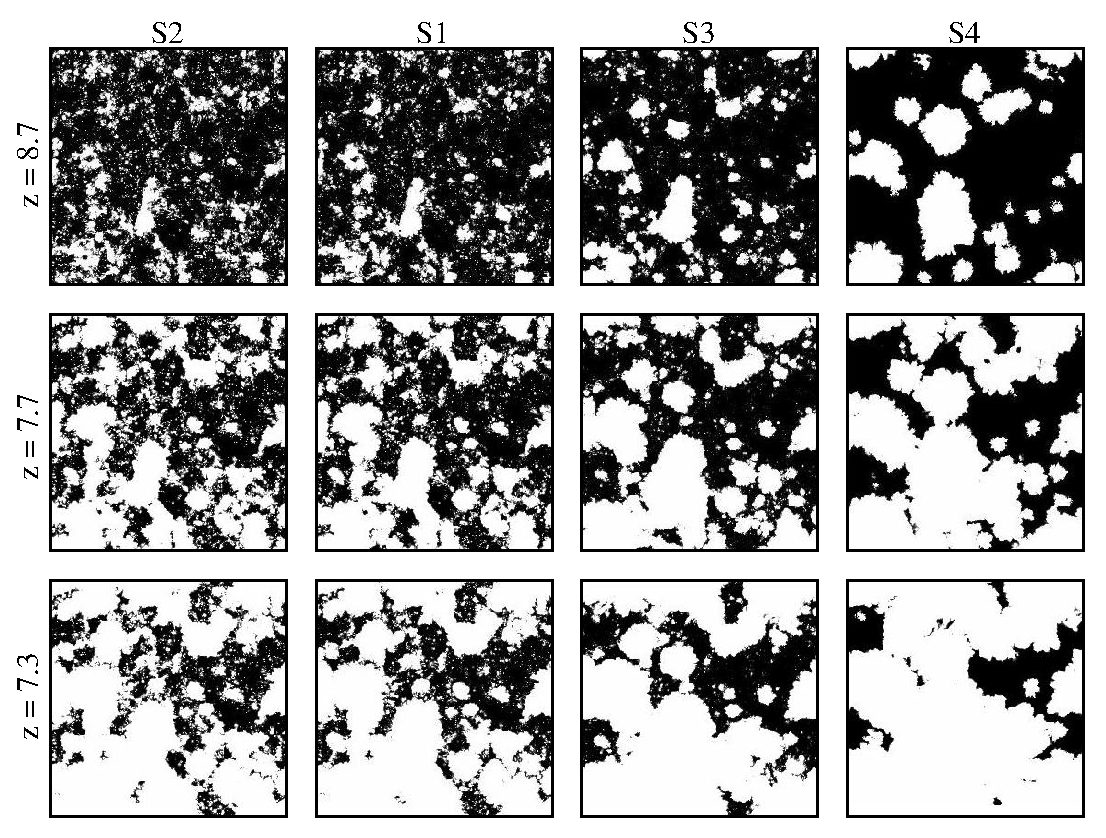
\includegraphics[width=6in]{chap0_intro/mcquinn_ionized_region_sims.eps}
	\caption[Four different simulations of the ionization field as a function of time.]{Four different simulations of the ionization field (columns) as a function of time (rows) during reionization. Reproduced from \citet{McQuinn06}}
	\label{fig:mcquinneorsims}
\end{figure}



\subsection{Simulations of the 21\,cm signal}
\subsubsection{The global signal}
\label{sec:globalsignal}

In this section we review the mean 21\,cm signal over cosmic time. Note first that the brightness temperature of the 21\,cm signal is determined by the spin temperature, which is affected by three processes: (1) collisional coupling with atoms and free electrons which couple the gas kinetic temperature to the spin temperature; (2)  radiative coupling to the CMB; and (3) Ly$\alpha$-induced spin-flips via an excited state. 

As the universe evolves, the relative importance of each of these processes changes, and the spin temperature evolves accordingly. Fig. \ref{fig:pritchardloebtemperatures} shows the gas, spin, and CMB temperatures (top), the ionized fraction (center), and the differential 21\,cm brightness temperature (i.e., the 21\,cm spin temperature relative to the CMB (bottom) as a function of redshift. Three different reionization models, giving different spin and differential brightness temperature histories are presented. At $1100>z>200$ (A), the universe is dense enough that Compton scattering holds $T_\text{gas}\approx T_\gamma$, and collisional coupling sets $T_s\approx T_\text{gas}$, so the relative 21\,cm brightness temperature is close to zero. Then over $200>z>50$ the gas cools adiabatically, implying\footnote{Adiabatic cooling implies $PV^\gamma=$const, where $\gamma=c_p/c_v=1+1/c_v$. For a monotonic ideal gas, the specific heat at constant volume is given by $c_v=3/2$. Note also that $TV^{\gamma-1}=$const, which gives $T\sim (1+z)^2$} $T\sim (1+z)^2$. The spin temperature thus cools a factor of $1/(1+z)$ faster than the CMB, so the differential brightness temperature becomes negative (B). Note that the gas is cooling below the CMB temperature, but the gas temperature is still coupled to the spin temperature because of collisions. At these high redshifts, structure is still largely linear, so that the brightness temperature traces the matter density field without corrupting the contaminating effect of \textit{gastrophysics}\footnote{Gastrophysics is a neologism referring to the astrophysical (i.e., non-cosmological) effects on the 21\,cm signal due especially to non-linear galaxy formation and feedback effects which are challenging to model.} 

\begin{figure}
	\centering
	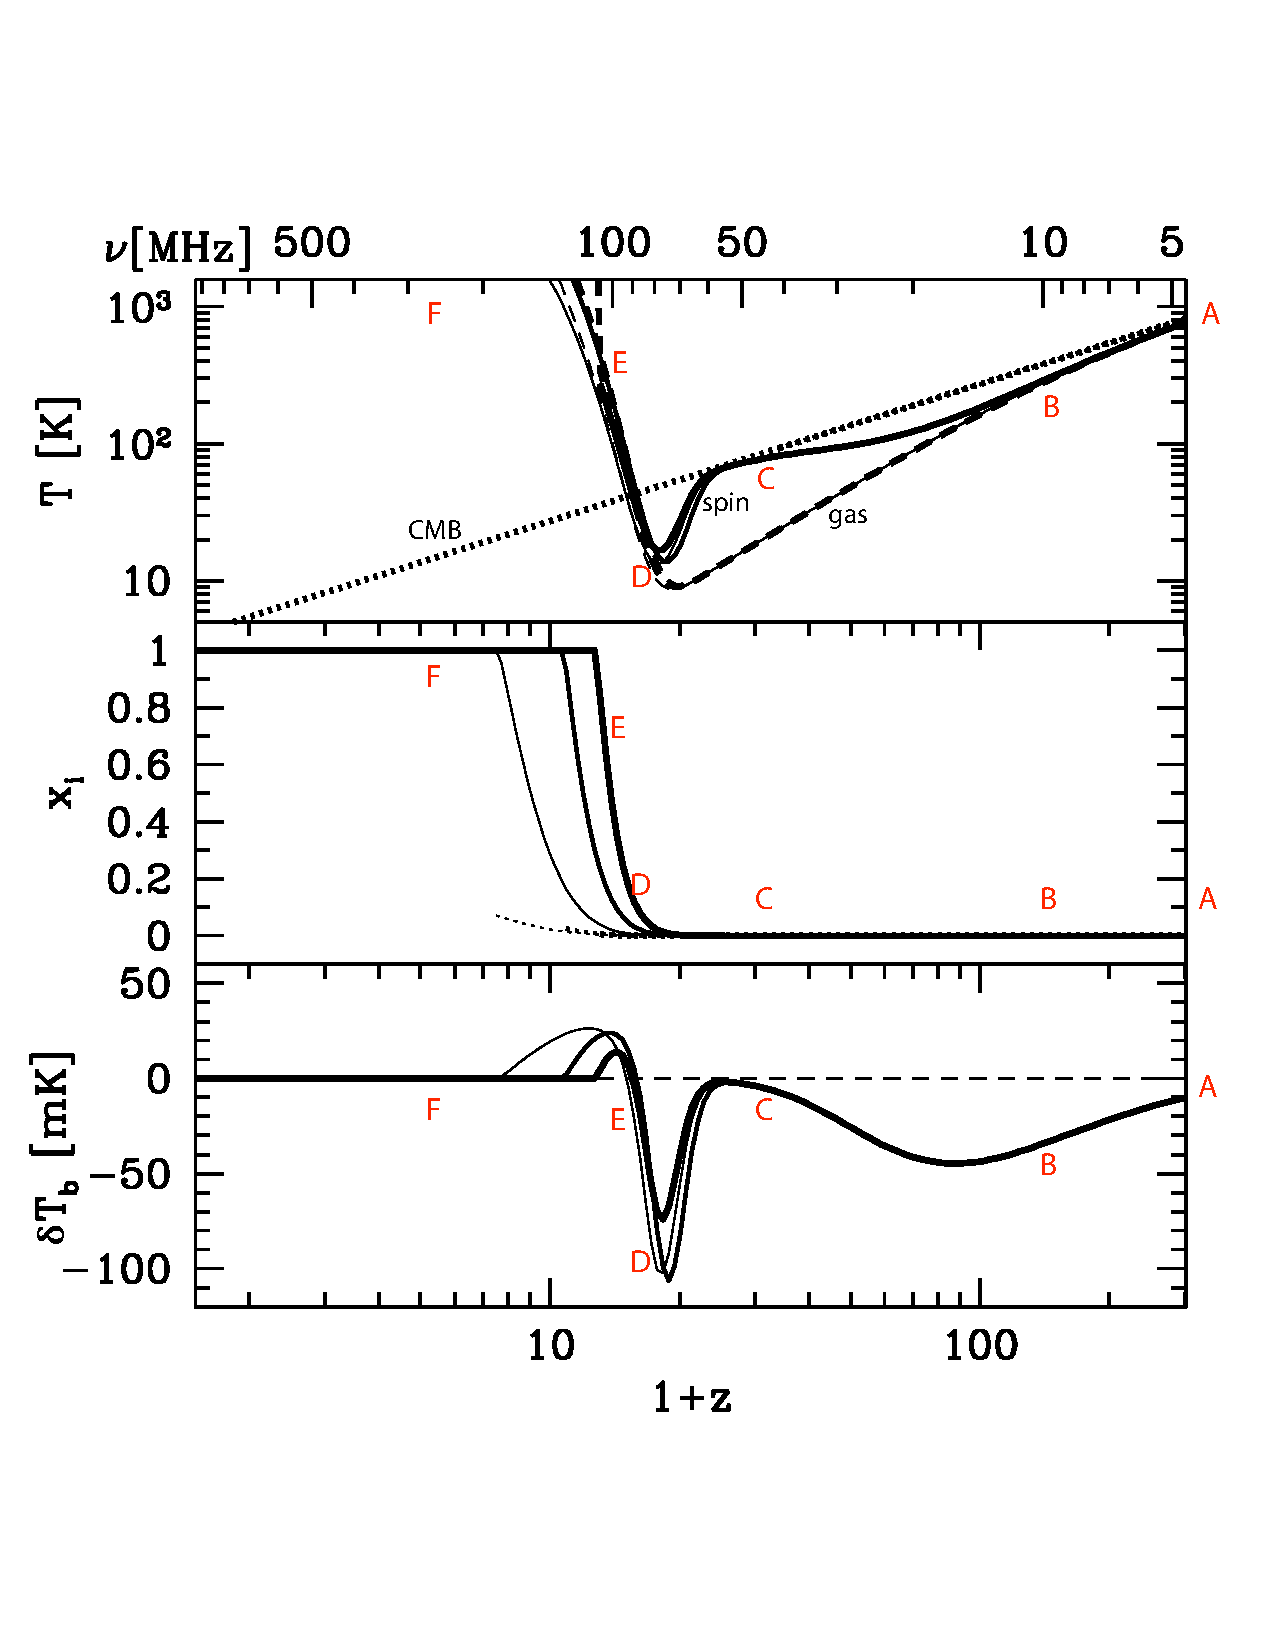
\includegraphics[width=6in]{chap0_intro/pritchard_and_loeb_temperatures_annotated.pdf}
	\caption[The spin, gas, and CMB temperatures, the ionization fraction, and the 21\,cm brightness temperature for three different reionization models.]{These panels show the spin, gas, and CMB temperatures (top), the ionization fraction (center), and the 21\,cm brightness temperature for three different reionization models. See Sec. \ref{sec:globalsignal}. Reproduced from \citet{PritchardLoebReview}}
	\label{fig:pritchardloebtemperatures}
\end{figure}

From here on, the exact sequence of events becomes quite uncertain. It is thought that as the universe continues to expand, the gas becomes too dilute for collisions to couple the gas and spin temperatures, and the spin temperature falls back into equilibrium with the CMB, reducing the differential brightness temperature towards zero (C). When the first sources form and begin to emit ionizing radiation, the Ly$\alpha$-induced spin flips mentioned above couple the spin temperature back to the gas temperature, which at this point is much colder than the CMB (D). In quick succession, heating of the IGM from this radiation becomes significant, raising the 21\,cm signal over the CMB temperature (E), until the bulk of the universe becomes ionized and there are no further large neutral regions to emit 21\,cm radiation (F).

\subsubsection{The power spectrum}

While the 21\,cm global signal encodes the galaxy formation and reionization history in the mean brightness of HI emission as a function of redshift, the power spectrum probes the state of the universe at a given redshift in more detail. In the  future, observations with the SKA-Low may be able to image the ionization field (Fig. \ref{fig:mcquinneorsims} directly, but current experiments such as the MWA, PAPER, HERA, LOFAR, and GMRT are pursuing power spectrum measurements\footnote{A cosmologist might even argue that \textit{only} power spectrum measurements are of interest, given that the primordial matter power spectrum is a prediction of inflation whereas the particular realization of the power spectrum that we observe has no fundamental significance. The 21\,cm power spectrum, however, is influenced by many astrophysical processes during the epoch of reionization, and its fundamental statistics are likely not entirely reducible to a simple power spectrum.} of the ionization field. The spatial power spectrum quantifies the amount of fluctuation power at different spatial scales, and by combining the information in many noisy pixels together, it can be sensitive to a 21\,cm signal even when none is apparent in the image. 

Fig. \ref{fig:fiducialPS} shows simulations of the 21\,cm brightness power spectrum by \citet{BarkanaPS2009} at points throughout the epoch of reionization. The power spectrum is plotted in units of $\Delta(k)=\sqrt{k^3 P(k)/2\pi^2}$. At the start of reionization (10\% ionization, yellow curve) tiny ionized bubbles have begun to form around the first galaxies, producing a point-source like power spectrum with $P(k)\propto$const, and thus $\Delta(k)\propto k^{1.5}$. As the bubbles grow, power shifts from large to small scales. At the end of reionization (98\% ionization, gray line), the bubbles merge into each other, ionizing the whole volume of space, and the 21\,cm signal drops off.

\begin{figure}
	\centering
	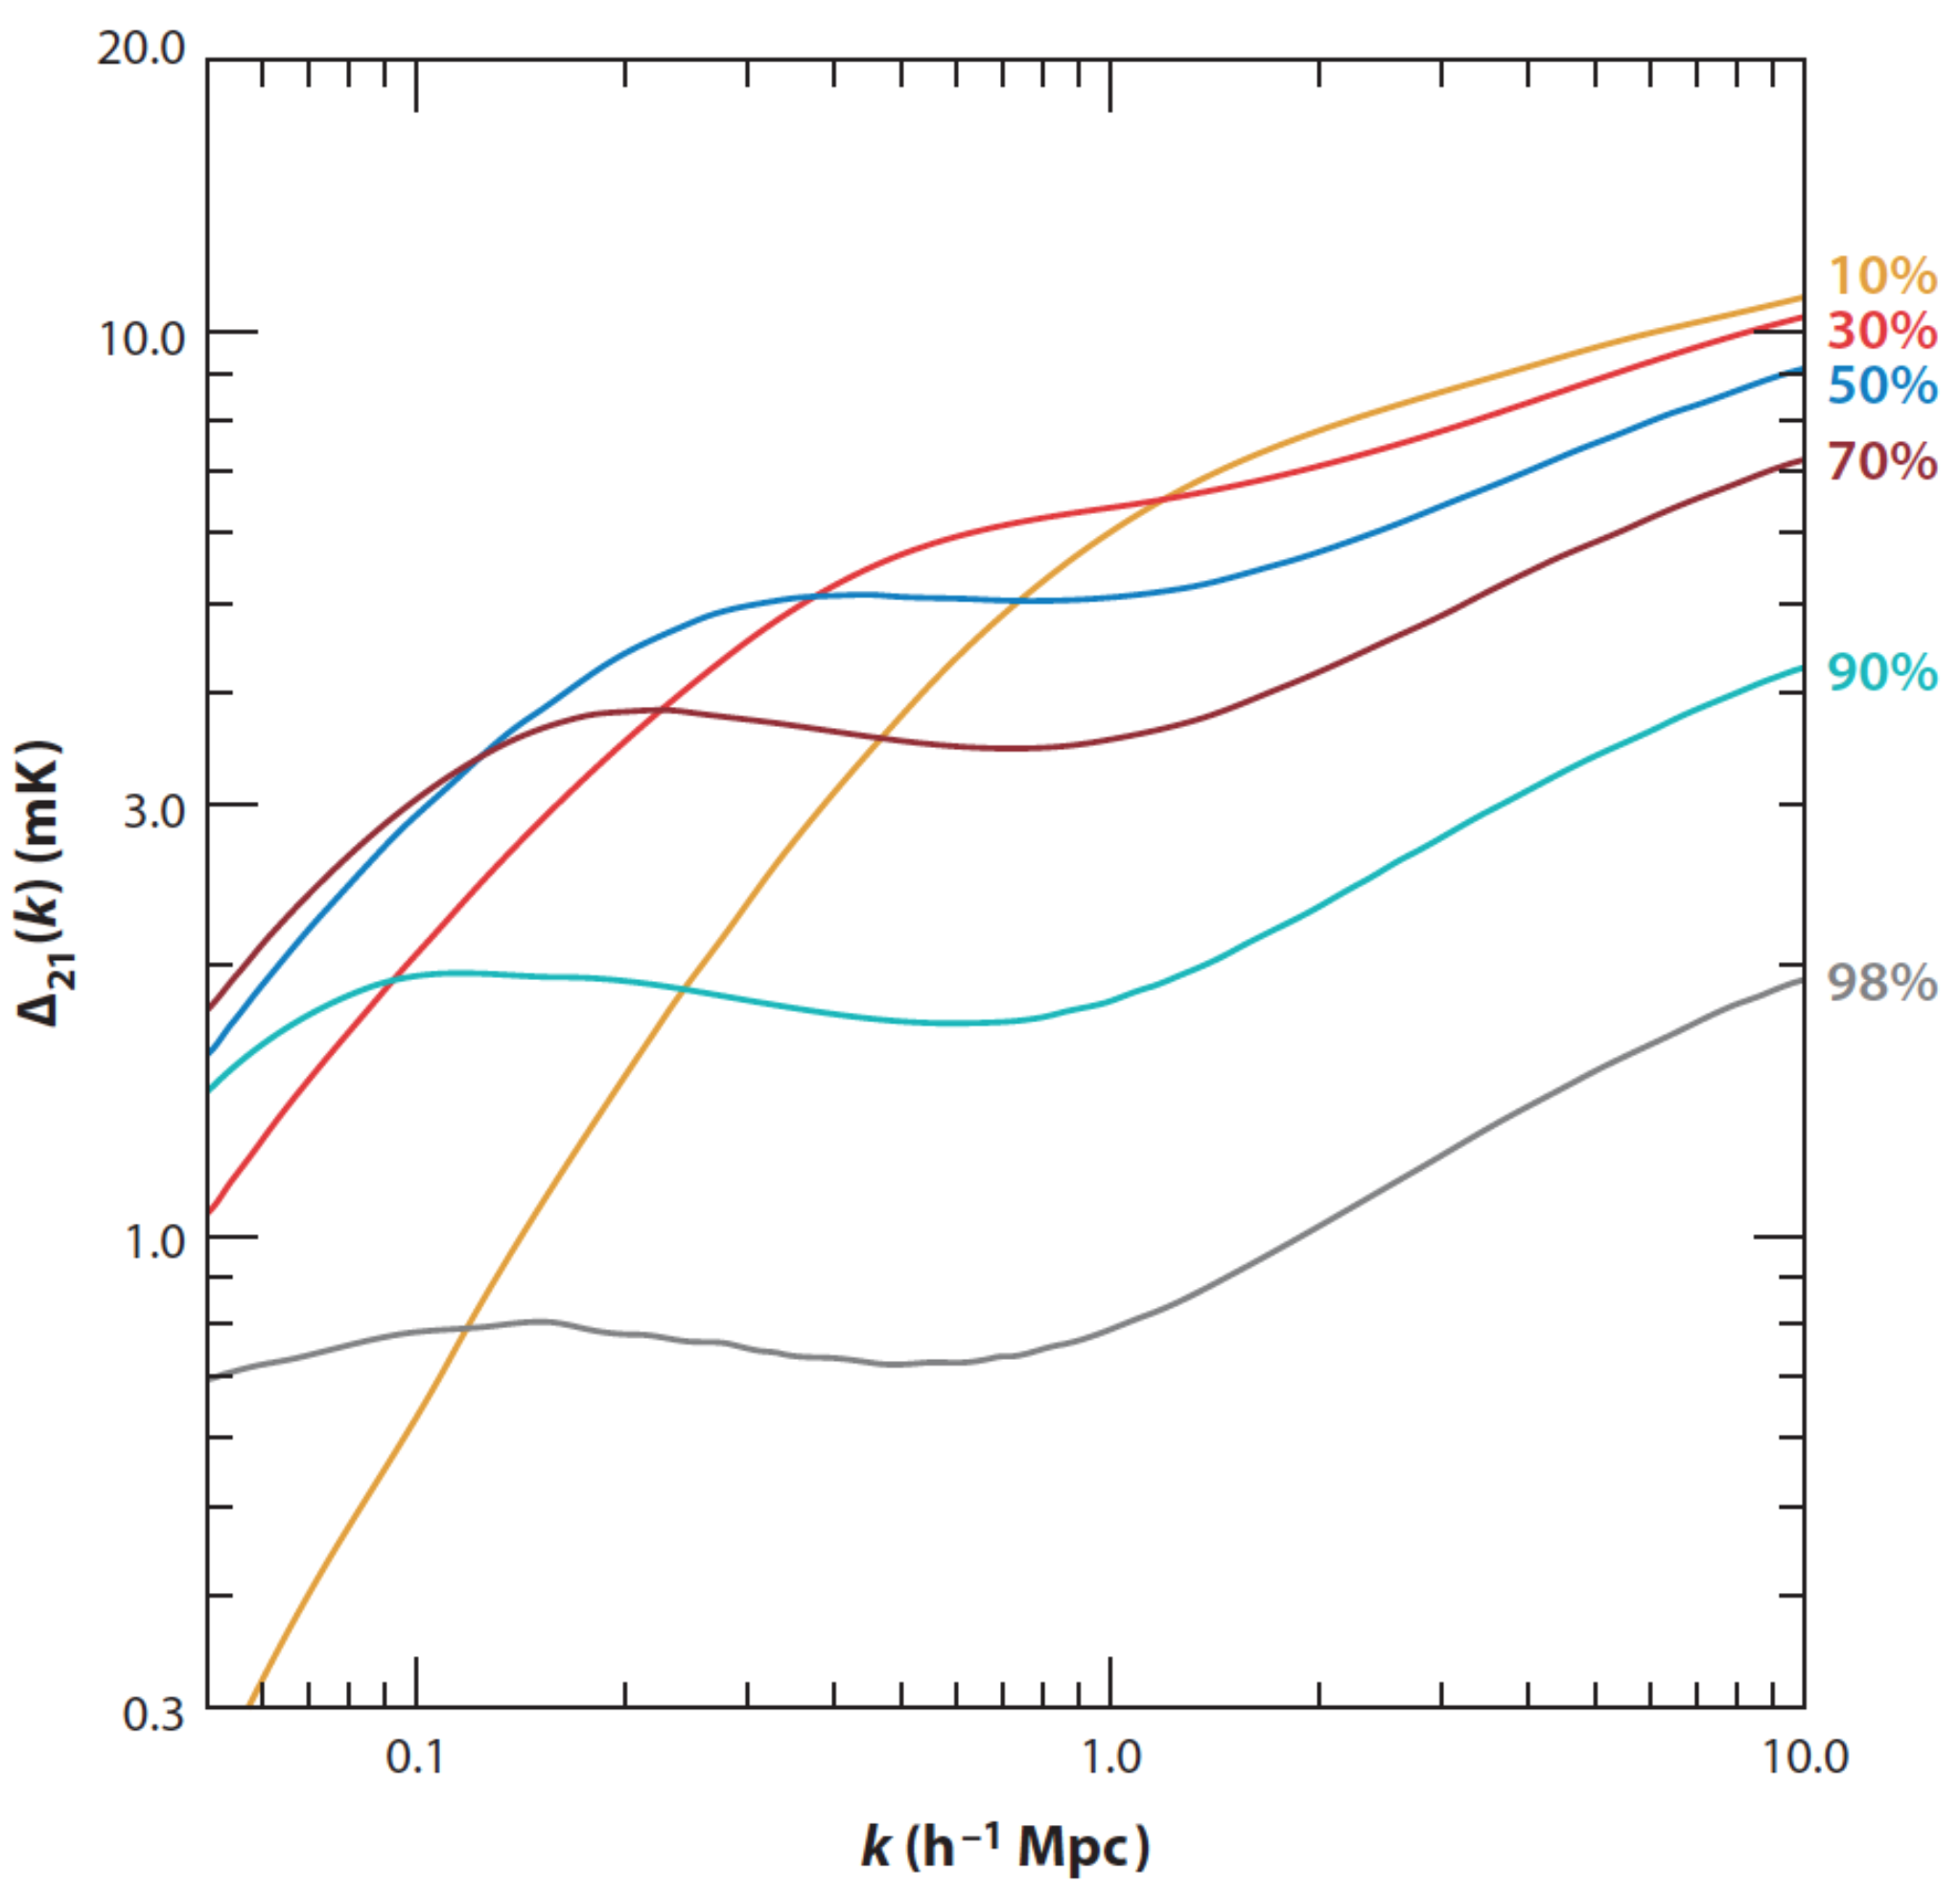
\includegraphics[width=4.5in]{chap0_intro/FiducialPS.png}
	\caption[Simulated 21\,cm power spectra at various points during the epoch of reionization.]{Simulated 21\,cm power spectra at various points during the epoch of reionization. As ionized bubbles grow around the first galaxies, spatial power shifts from small to large scales, and the signal eventually drops off at the end of the EOR as the whole volume of space becomes ionized. Reproduced from \citet{BarkanaPS2009}}
	\label{fig:fiducialPS}
\end{figure}

\section{Measuring the 21\,cm signal with radio interferometers}

\subsection{The basics of radio interferometry}

A radio interferometer is an array of separate antennas whose outputs are correlated with each other, and combined to form an image. It is ofter cheaper and easier to use such a ``synthetic aperture'' to improve resolution and collecting area than to simply build ever bigger single dish antennas, especially given advances in computing permitting real time correlation of hundreds of antennas. In this section I will review how we get from the individual antenna outputs to a sky image for a simple 1D array viewing a 1D sky.

\begin{figure}[h]
    \centering
    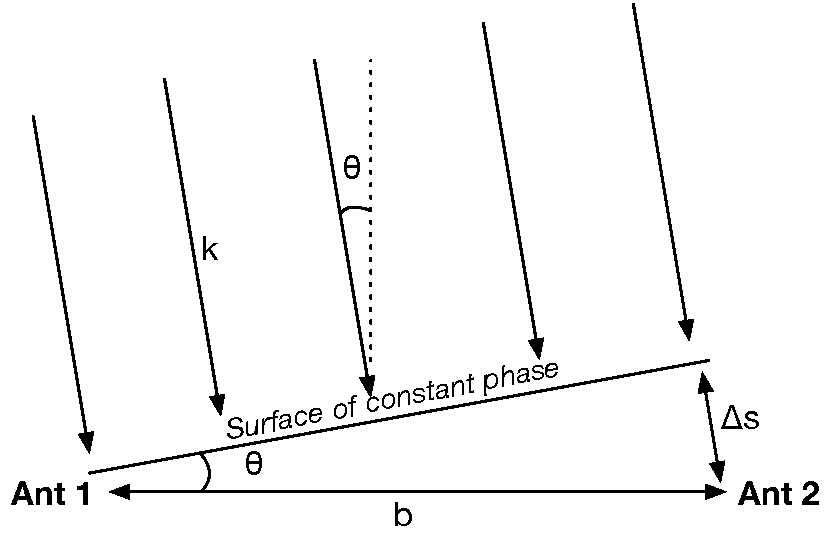
\includegraphics[width=0.95\textwidth]{chap0_intro/radio_interferometer_diagram.pdf}
    \caption[Diagram of a two element radio interferometer]{A single baseline (i.e., pair of antennas) displaced by $b$ on the ground receive radiation from a distant source at an angle $\theta$ from zenith. The source is distant enough that its surfaces of constant phase are planes which are orthogonal to $\vec{k}$, the wavevector of the radiation. The radiation arriving at Antenna 1 accumulates extra phase due to the path length difference $\Delta s$ compared to that arriving at Antenna 2.}
    \label{fig:radiointerferometerdiagram}
\end{figure}

Consider first a pair of antennas (termed a \textit{baseline}) on the ground separated by distance $b$. Radiation arrives from a distant source at an angle $\theta$ from zenith. Observe (Fig. \ref{fig:radiointerferometerdiagram}) that after the surface of constant phase reaches the first antenna, it must propagate an extra distance $\Delta s$ before reaching Antenna 2, acquiring an extra phase of $\vec{k}\cdot \vec{b}=2\pi\Delta s/\lambda=2\pi\sin b/\lambda$. Then the time averaged cross correlation between the voltages measured at antenna 1 and 2, known as the visibility $V_{12}$, is
\begin{equation}
\label{eqn:vis1D}
	V_{12}\equiv\langle V_1(t)V_2^*(t)\rangle=\langle(V_0 e^{i\omega t})(V_0^*e^{-i(\omega t-2\pi u\sin \theta)})\rangle = |V_0|^2 e^{2\pi i u\theta}
\end{equation}
using the small angle approximation and measuring the baseline length in units of wavelengths $u\equiv b/\lambda$. We can see that $u$ and $\theta$ are fourier dual variables. If we can measure the visibility at many different baseline lengths, then we can grid them in $u$ space and take the fourier transform to get their representation in the $\theta$ space, i.e., the sky image.

\begin{figure}[h]
    \centering
    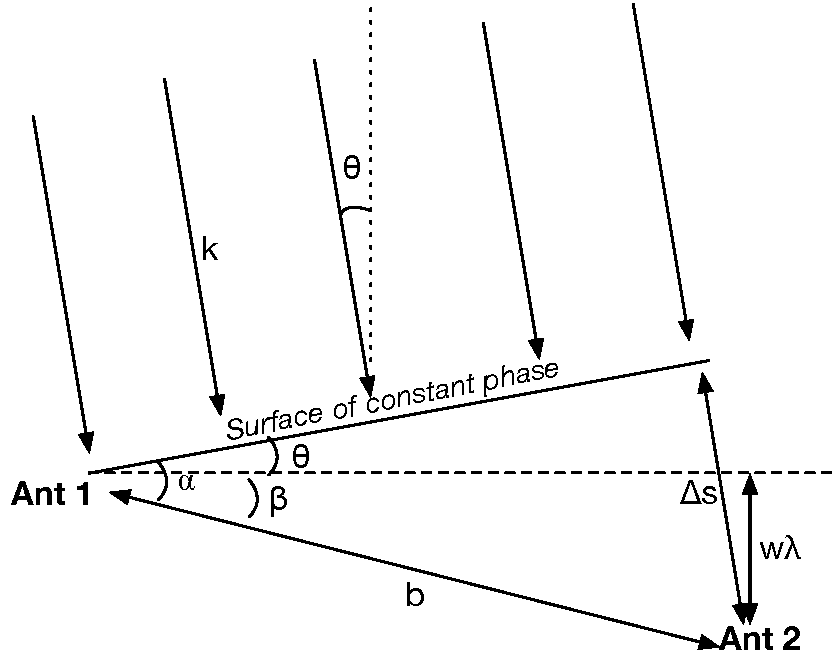
\includegraphics[width=0.95\textwidth]{chap0_intro/radio_interferometer_diagram_with_w.pdf}
    \caption[Diagram of a two element radio interferometer with non-zero $w$.]{Diagram of a two element radio interferometer as in Fig. \ref{fig:radiointerferometerdiagram} but with the baseline not necessarily in the plane orthogonal to zenith.}
    \label{fig:radiointerferometerdiagramwithw}
\end{figure}

Let's consider one higher level of detail where the baseline is not necessarily in the plane orthogonal to zenith, as Fig. \ref{fig:radiointerferometerdiagramwithw}. 
We are still assuming a 1D sky. As before, the visibility due to a source at angle $\theta$ from zenith is given by $|V_0|^2 e^{2\pi i \Delta s/\lambda}$. 
The extra path length is given by $\Delta s=b\sin\alpha=b\sin(\theta+\beta)$, where $\beta\equiv\arcsin (\text{w}\lambda/b)$ is the angle between the baseline and the plane orthogonal to zenith. 
We also define $\ell\equiv\sin\theta$, and
 $u\equiv (b/\lambda)\cos\beta$, 
 so that $\sqrt{u^2+\text{w}^2}=b/\lambda$. 
 Putting all this together gives
\begin{eqnarray}
	\frac{\Delta s}{\lambda} &=& \frac{b}{\lambda}\sin\left[\theta+\arcsin\left(\frac{\text{w}\lambda}{b}\right)\right]\\
	 &=& \frac{b}{\lambda}\sin\theta\cos\beta+\text{w}\cos\theta\\
	 &=& u\ell+\text{w}\sqrt{1-\ell^2}
\end{eqnarray}
And the full expression for the visibility on baseline (u,w) due to a source at $\theta$ away from zenith becomes 
\begin{equation}
	V(u,w)=|V_0|^2 e^{2\pi i (u\ell+\text{w}\lambda\sqrt{1-\ell^2})}
\end{equation}
where $|V_0|^2$ is proportional to the power received from that source through a constant determined during calibration. 

Generalizing this for a 1D sky with an intensity distribution per angle of $I(\ell)$ we have $V(u,w)=\int I(\ell)e^{2\pi i (u\ell+\text{w}\lambda\sqrt{1-\ell^2})}d\theta$. Note that $\ell=\sin\theta$, implying that $d\ell=\cos\theta d\theta$, and thus that $d\theta=d\ell/\sqrt{1-\ell^2}$. This gives the final expression for a visibility in our 1D case.
\begin{equation}
V(u,w)=\int I(\ell)e^{2\pi i (u\ell+\text{w}\lambda\sqrt{1-\ell^2})}\frac{d\ell}{\sqrt{1-\ell^2}}
\end{equation}

Note that $\text{w}\neq0$ disrupts the simple Fourier relationship between $u$ and $\ell\equiv\sin\theta\approx\theta$ we observed in Eqn. \ref{eqn:vis1D}. We term baselines with $\text{w}\neq0$ \textit{non-coplanar}, and we will comment further on how they affect imaging algorithms at the end of this section.

Treating the more general case of a 2D sky gives 
\begin{equation}
V(u,v,w)=\int I(\ell,m)e^{2\pi i (u\ell+vm+\text{w}\lambda\sqrt{1-\ell^2-m^2})}\frac{d\ell}{\sqrt{1-\ell^2-m^2}}
\end{equation}
where $\ell$ and $m$ are the sines of the angles in orthogonal directions away from zenith, and $u$ and $v$ are the components of the baseline in the plane orthogonal to zenith measured in units of wavelengths \citep{thompsonmoranswenson}. Note that in fact these equations do not require $u$ and $v$ to be defined relative to zenith, we could instead compute them as components of the baseline in the plane orthogonal to an arbitrary \textit{phase center}. In that case, $w$ would be the component in the direction of that phase center. For instance, in a interferometer with steerable dishes, it typically makes sense to choose the phase center of the analysis to coincide with the pointing center of the dishes. 

Real world interferometers have non-uniform and incomplete sampling in $u$ space, encoded by a sampling function $S(u)$. We may view this function as a sum of delta functions located at all the sampled $u$ values: $S(u)=\sum_{i,j}\delta(u_i-u_j)$, where $i,j$ index the antennas. Multiplying the true visibility function $V(u)$ by this sampling function, then fourier transforming, is equivalent (by the convolution theorem) to convolving the true sky image by the fourier transform of the sampling function, known as the synthesized beam. This is known as the \textit{dirty image}. Unlike in optical astronomy where the point spread function is close to a gaussian or an Airy function, the synthesized beam is generally non-compact with significant sidelobes due to sparse baseline sampling.  

The strategy is typically to distribute the antennas pseudo randomly to achieve as many different baselines as possible, calculate the dirty image, then use an iterative procedure known as CLEAN \citep{hogbomclean} and its variants to incrementally deconvolve the synthesized beam from the true sky image. This procedure makes the often valid assumption that the true sky is simply a collection of isolated point sources. The statistics of the resulting \textit{clean image} are difficult to quantify as CLEAN is a non-linear algorithm, but in practice it is found to work quite well and is indispensable to characterizing the compact radio sources between us and the EOR signal (i.e., \textit{foregrounds}). A last note is that a number of methods have been developed to treat the non-coplanar baselines effect which disrupts the simple fourier relationship between baseline space and image space, the most popular of which is an extension of CLEAN known as w-projection \citep{wproj}.

%There are several methods to deal with the w-term during imaging: faceting (Cornwell & Perley 1992); a three-dimensional Fourier transform (Perley 1999); ; w-stacking (Humphreys & Cornwell 2011); and warped snapshots (Perley 1999). Hybrid methods are sometimes useful, such as with the w-snapshots method (Cornwell, Voronkov & Humphreys 2012).

\subsection{From image cubes to power spectra}

First generation experiments lack the sensitivity to directly image 21\,cm emission from the EOR, and aim instead at statistical detections of the signal which combine many low SNR pixels into a significant statistic. The most prominent of these methods is estimation of the power spectrum.

To understand how cosmological power spectrum measurements are made, let us first consider the space that the interferometer measurements reside in. The fundamental measurements are cross correlations, also known as visibilities, at different frequencies. We have shown in the previous section that each visibility is a measure of a different sky fourier mode $(u,v)$, coordinates which are dual to $(\theta_x,\theta_y)$. However, each frequency corresponds to a different cosmological redshift, and thus, distance from us. Interferometric visibilities thus live in an awkward mixed fourier space. To study foregrounds, we must fourier transform along $u$ and $v$ to reach 3D image space, but to make power spectrum measurements, we must transform along $f$ to reach 3D fourier space. This is illustrated in Fig. \ref{fig:ifospace}, where we denote the fourier dual to $f$ as $\eta$, termed \textit{delay}.

\begin{figure}[h]
    \centering
    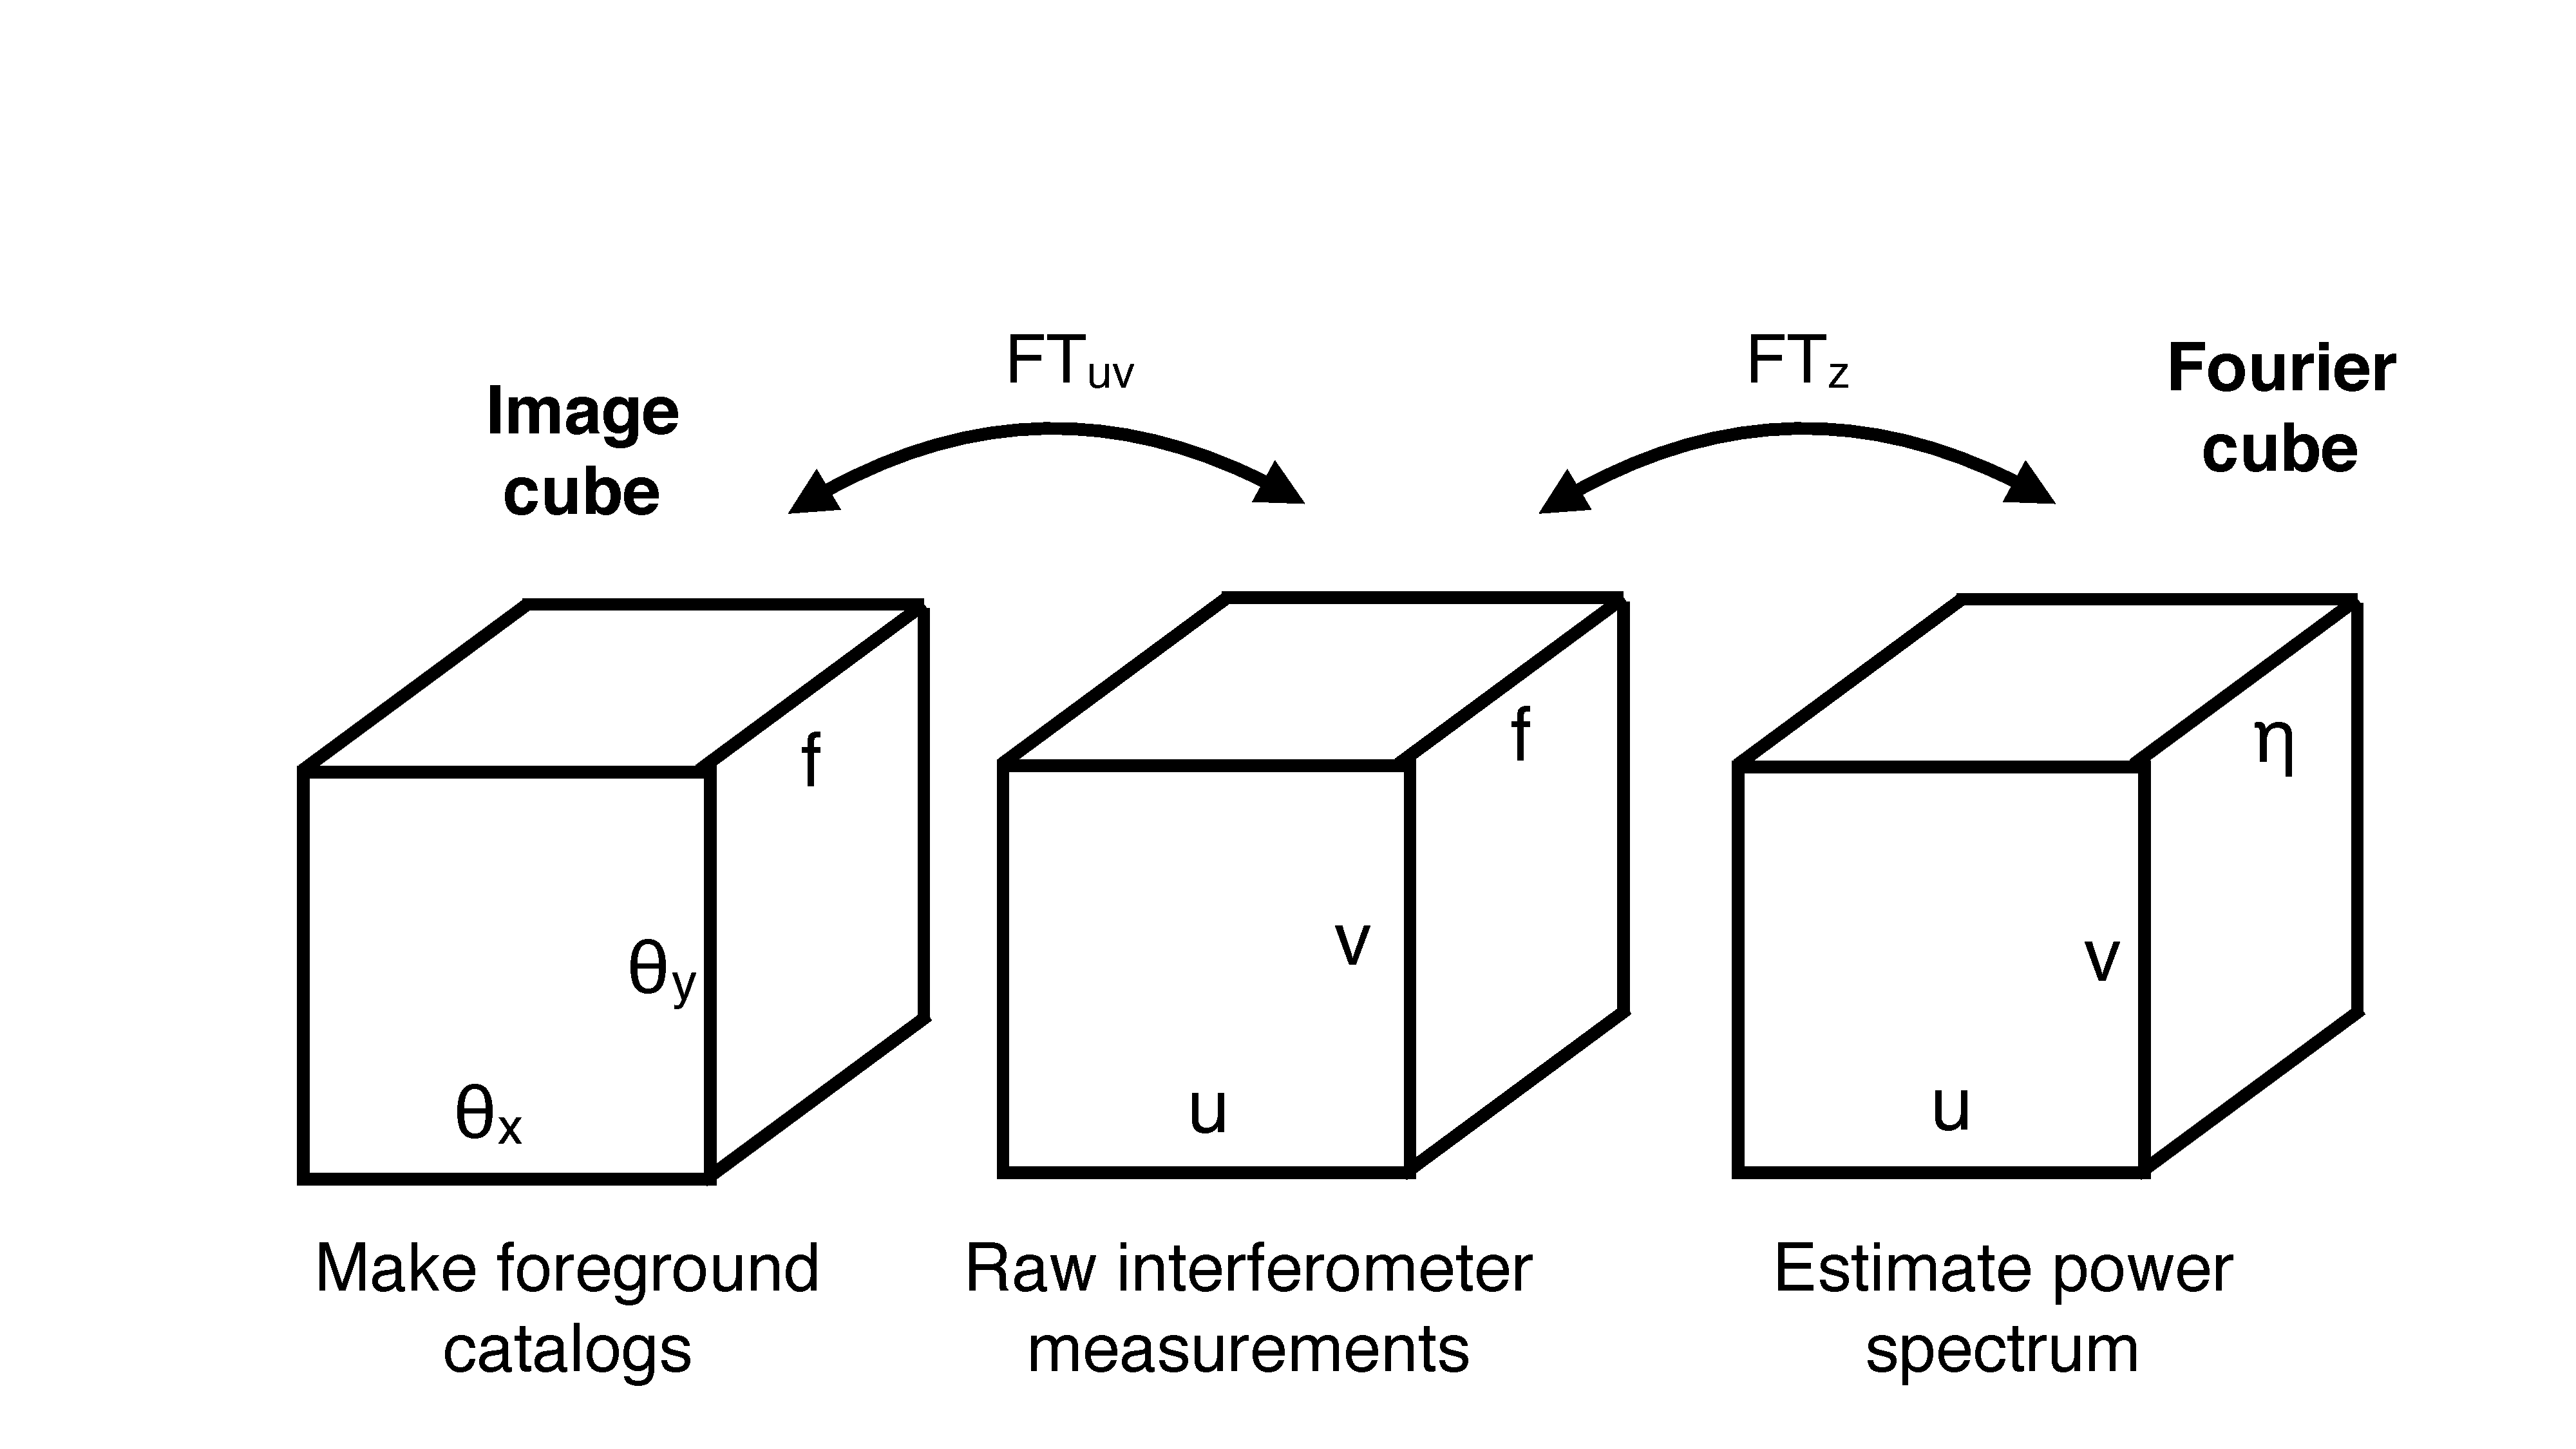
\includegraphics[width=1\textwidth]{chap0_intro/ifo_space.pdf}
    \caption{Representation of the relation between image space (left), fourier space (right), and interferometer space (center).}
    \label{fig:ifospace}
\end{figure}

We seek to estimate the spatial power spectrum of 21\,cm emission in comoving units, that is, as a function of wave number $k$ with units of inverse comoving distance. We must first rescale $u$ and $v$ to $k_x$ and $k_y$. For brevity, consider only the $x$ dimension. $u$ is defined by the fourier factor $e^{2\pi i u\theta}$, which we must match with $k_x$, defined by $e^{ik_x x}$, where $x$ is the comoving distance transverse to the line of sight. Setting their exponents equal and using $x=D\theta$, where $D$ is the transverse comoving distance to the redshift of interest, we find.

\begin{eqnarray}
	k_x=\frac{2\pi u}{D} \\ 
	k_y=\frac{2\pi v}{D} \\ 
\end{eqnarray}

To relate $k_z$ to $\eta$, we must first match the exponents in $e^{i k_z x_\parallel}$ and $e^{i\omega \eta}$, where $x_\parallel$ is the comoving distance along the line of sight\footnote{Unfortunately we can't refer to this as $z$ because it's taken by the cosmological redshift.} and $\omega=2\pi f$ gives the observation frequency. Matching these, and using that $d x_\parallel/df=cf_0/H(z)f^2$, we find

\begin{equation}
	k_z=\frac{2\pi\eta f_0 H(z)}{c(1+z)^2}
\end{equation}

\begin{figure}[h]
    \centering
    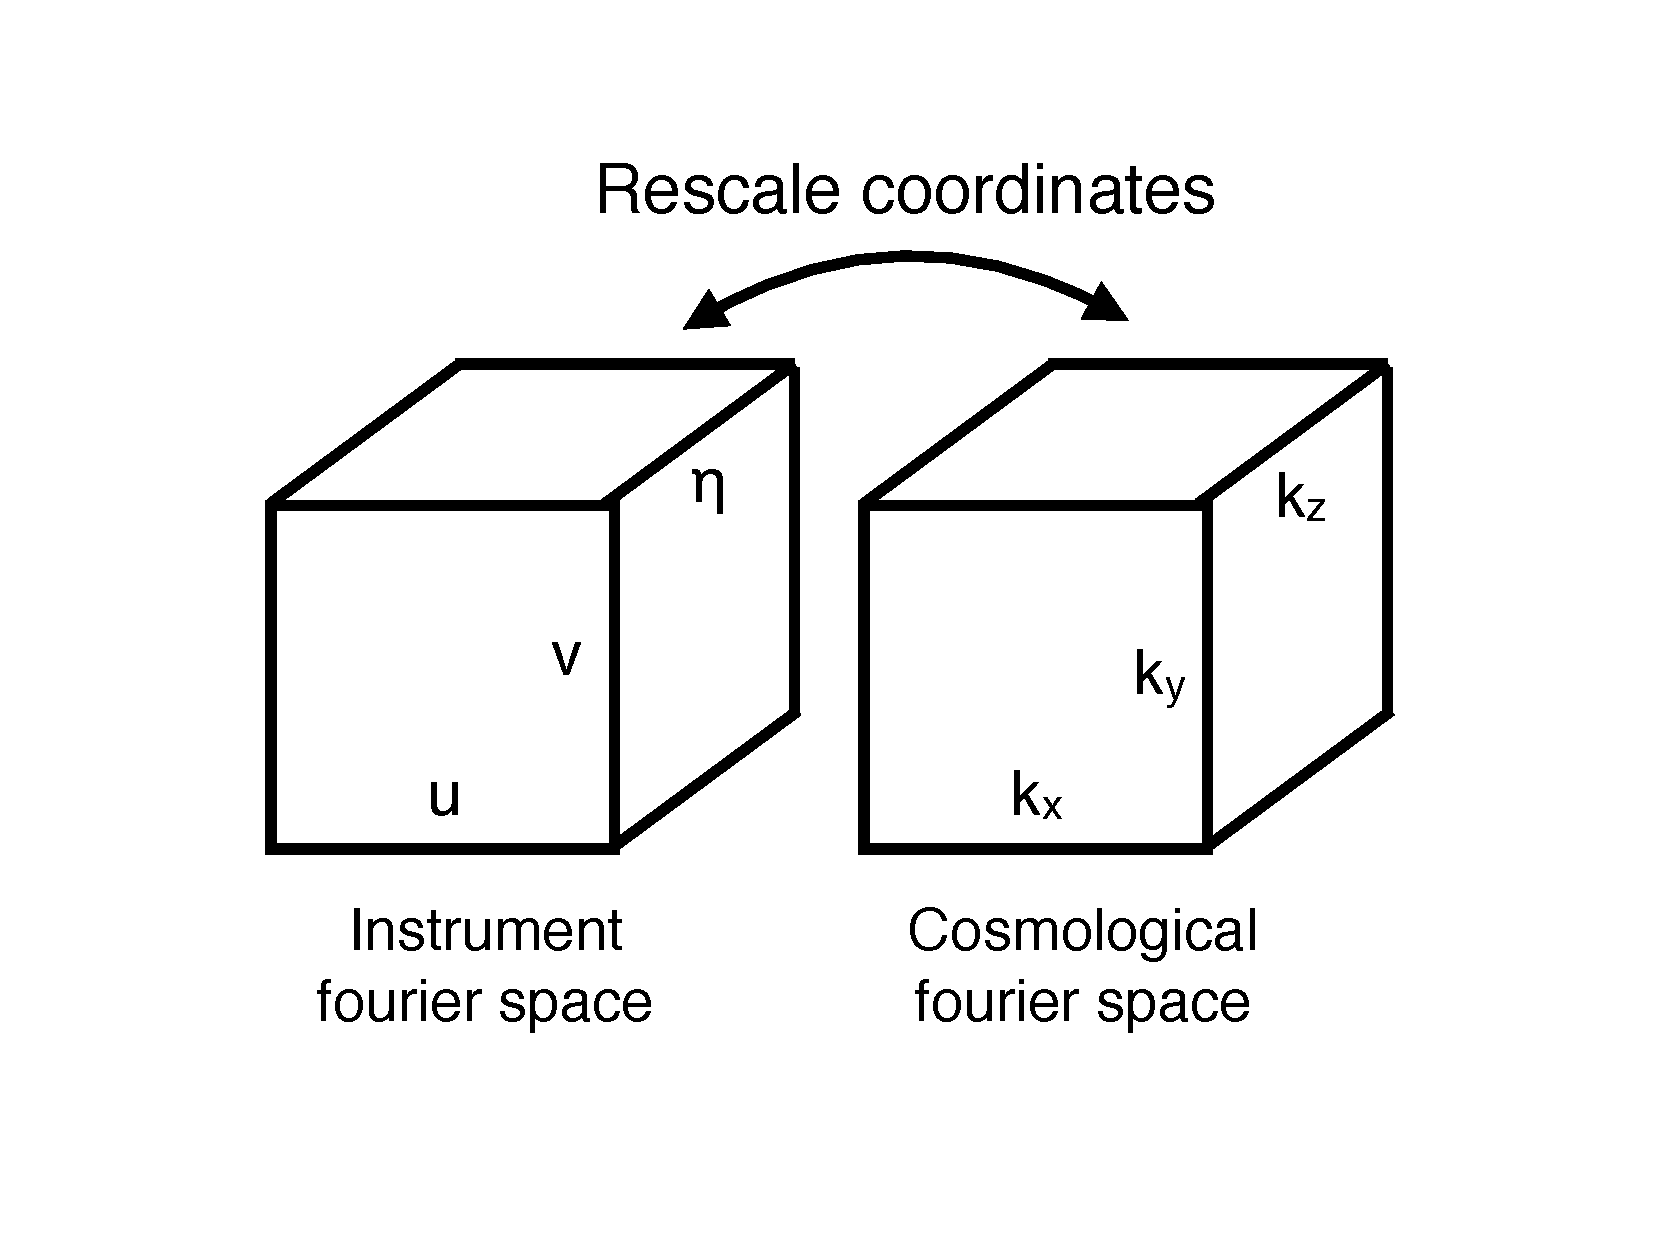
\includegraphics[width=0.9\textwidth]{chap0_intro/ifo_space_cosmo.pdf}
    \caption{Representation of the rescaling between instrument fourier space and cosmological fourier space.}
    \label{fig:ifospacecosmo}
\end{figure}

A last note is that to characterize foregrounds, we often combine $k_x$ and $k_y$ together to plot the 2D \textit{cylindrically} binned power spectrum as a function of $k_\perp\equiv(k_x^2+k_y^2)^{1/2}$ and $k_\parallel\equiv k_z$.

%optimal quadratic power spectrum estimators, essentially, generalized FT with arbitrary weighting



\subsection{Sensitivity challenges}
\label{sec:sensitivity}

The two major challenges to observing redshifted 21\,cm emission from the dark ages and EOR are noise and foregrounds. Interferometers at low frequencies are sky noise dominated, meaning that the diffuse galactic synchrotron dominates the received antenna power, and thus, the visibility noise. However it is so diffuse, and thus, so compact in $uv$ space, that its contribution to the mean visibilities is negligible. See Appendix A for a detailed discussion of sky noise. Our concern here is that even in the coolest parts of the sky, at high galactic latitudes, galactic synchrotron has brightness temperatures of $\sim200$\,K \citep{Tsysmemo}. The cosmological global signal is at the tens of mK level, and simulations suggest that individual fourier modes are far smaller, at the few mK level. 

Let us get a sense for the sensitivity challenge with a rough calculation. I show in Appendix A that the noise $\sigma_V$ on visibility $V_{ij}$ is given by $V_{ii}/\sqrt{Bt}$ where $V_{ii}$ is the autocorrelation, $B$ is the bandwidth, and $t$ is the observation time. Measuring the sky in brightness temperature units, the autocorrelation is given by $V_{ii}=\int T(\hat\theta)d\Omega\sim T_\text{sky}\Omega$, where $\Omega=\lambda^2/A$ is the solid angle of the beam main lobe. Comparing this brightness temperature noise with the expected few mK cosmological visibilities, gives roughly 100 hours for a 5$\sigma$ detection. 

However, we don't need a 5$\sigma$ detection in every visibility to detect the power spectrum. Consider a simple case where we neglect the frequency dimension. Let raw visibilities have noise $\sigma_V$, and let each $uv$ cell be the average of $N_\text{vis.per.cell}$ of them. Then the power spectrum is is estimated by averaging the power over the $N_\text{cells}$ cells with similar $\sqrt{u^2+v^2}$ magnitude. The noise on the mean visibility $\bar{V}$ in each cell is $\sigma_{\bar V}=\sigma_V/\sqrt{N_\text{vis.per.cell}}$, and the noise on its square can be shown to be $\sigma_{\bar |V|^2}\sim\sigma_{\bar V}^2\sim\sigma_V^2/N_\text{vis.per.cell}$, which is reduced by $1/\sqrt{N_\text{cells}}$ when spherically binning. So we find 

\begin{equation}
	\sigma_P\propto\frac{\sigma_V^2}{N_\text{vis.per.cell}\sqrt{N_\text{cells}}}
\end{equation}

Thus we see that there are two kinds of averaging which reduce the level of thermal noise in the power spectrum: \textit{coherent} averaging (by a factor of $1/N_\text{vis.per.cell}$) within individual $\vec{k}$ modes, and \textit{incoherent} averaging (by a factor of $1/\sqrt{N_\text{cells}}$) of power over different $\vec{k}$ modes falling into the same spherical $k$ bin. In the first case, we average different measurements of the same true value but with different noise, whereas in the second case, we average different realizations of the true spherical bandpower $k$. Were there no thermal noise on our measurements, the first average would do nothing, but the second would help to reduce sample variance noise. 

So we see that sensitivity of a real interferometer is set by the amount of coherent and incoherent binning of thermal noise, due to the 200\,K diffuse galactic synchrotron emission.  \citet{beardsley13} predict a $7\sigma$ detection of the power spectrum with the Murchison Widefield Array after 450\,hours, and \citet{PoberNextGen} predict a 3--7$\sigma$ detection after 1080\,hours, depending on foreground properties. In contrast to the MWA, whose antennas are distributed pseudo randomly to maximize the number of $uv$ modes sampled, PAPER's antennas are placed on a grid. Thus very few $uv$ modes are sampled, which makes imaging extremely challenging, but from a power spectrum point of view, they have optimized for coherent averaging at the expense of incoherent averaging. \citet{PoberNextGen} thus predict comparable sensitivities to the MWA despite their substantially smaller antennas. HERA builds on both sets of lessons learned, employing ultimately 350 14\,m dishes on a grid, and should yield tens of $\sigma$ detection \citet{neben16b,ewallwice16,nithya16,PoberNextGen,patra16}. 

\subsection{Foreground challenges}
\label{sec:foregroundchallenges}
While the diffuse synchrotron emission in our galaxy generates the noise on our measurements, compact extragalactic radio sources between us and the EOR generate a bias. We term these these sources \textit{foregrounds}, though the rest of the astronomy community terms them \textit{science}. Over the 100-200\,MHz band corresponding to redshifted 21\,cm emission from the EOR, foreground emission is sourced by radio synchrotron generated by relativistic electrons gyrating around galactic magnetic field lines as well as synchrotron from extragalactic jets. I derive in Appendix \ref{chap:synchrotron} that synchrotron emission has a power law spectrum with $I\sim\nu^{-0.75}$.

\begin{figure}
	\centering
	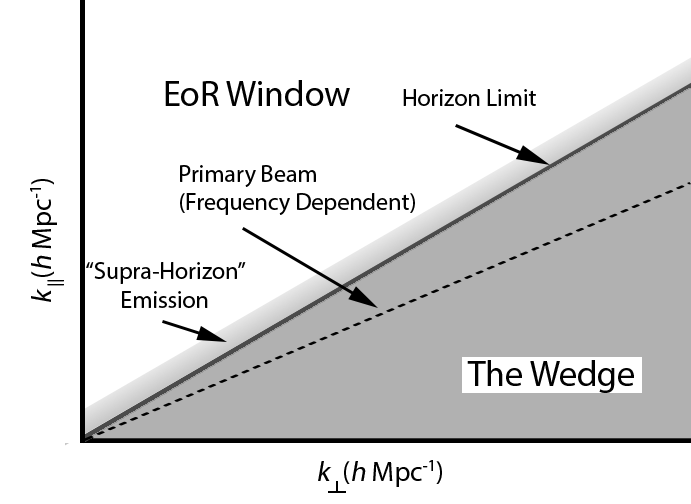
\includegraphics[width=5in]{chap0_intro/wedge-diagram.png}
	\caption[aeouaoeu]{Frequency-dependent sampling by interferometers imprints frequency dependence on otherwise smooth or flat spectrum foregrounds (see Sec. \ref{sec:foregroundchallenges}). This results in foreground contamination largely in a wedge-shaped region in $k_\parallel,k_\perp$ space, whose complement is termed the EOR window. Reproduced from \citet{dillonthesis2015}}
	\label{fig:wedgediagram}
\end{figure}

This smooth spectral structure of foregrounds is key to distinguishing them from the blotchy reionizing universe (Fig. \ref{fig:mcquinneorsims}). Any line of sight through the EOR will pass through some neutral regions and some ionized regions, all at slightly different redshift, and thus, frequencies. The sum spectrum, thus, should appear spectrally very unsmooth. Early work proposed removing smooth structure from every line of sight separately, subtracting splines, low order polynomials, or eigenforegrounds \citep{Judd08, paper1, paper2,xiaomin,LOFAR2,Harker,Jelic08,MoralesBowmanHewittFGsub}. However, simulations \citep{Dattapowerspec}, early theory \citep{VedanthamWedge,MoralesPSShapes,CathWedge,nithya13}, and early data reductions have shown that this is not the whole story. The frequency-dependent $uv$ sampling of interferometer baselines causes spectrally smooth foreground power to leak into higher $k_\parallel$ modes. Said differently, as a function of frequency, each baseline samples a different fourier mode of the sky, and that effect cannot be perfectly removed by simply gridding the baseline to a different $uv$ cell at different frequencies. Longer baselines move through $uv$ space faster with frequency, and after gridding many baselines, this linear dependence manifests as a wedge-shaped region (Fig. \ref{fig:wedgediagram}) in  $k_\perp,k_\parallel$ containing the nearly all foreground power. 

Work is ongoing to understand the slight leakage of foreground power outside of this region. \citet{AdrianWedge1,AdrianWedge2} show that it introduces not only biases power spectrum estimates but correlates error bars on wedge modes as well. It also manifests differently \citep{pober13} in the approximate power spectra computed using the per-baseline technique of \citet{parsonsandbacker,parsons12b} than in the image-based power spectra of \citep{beardsley16,dillonneben,X13}. 

Knowing this, two basic approaches to foreground removed have been discussed in the literature: foreground avoidance and foreground subtraction. The former consists of simply excluding modes in the wedge from power spectrum estimation, albeit at a significant loss of sensitivity, while the latter requires subtraction of 99.99\% of foreground intensity. Both are challenging, and neither has yet resulted in an EOR detection, but new experiments such as the under-construction HERA \citep{neben16,ewallwice16,nithya16,deboer16,patra16} and the next generation SKA \citep{ska,ska1,ska2,ska3} are taking note of all these lessons learned, and are predicted to yield highly significant detections in even the most pessimistic foreground cases. 

\subsection{A new generation of low frequency radio interefrometers}

In this section I will introduce the class of experiments being conducted to observe spatial fluctuations in 21\,cm emission from the EOR, and outline the experimental challenges they pose. As discussed in Sec. \ref{sec:sensitivity}, detection of 21\,cm emission from the EOR demands hundreds of hour integrations on arrays with hundreds of antennas. Even so, arrays such as MWA, PAPER, LOFAR, and now HERA are targeting only a statistical detection of the emission, that is, detection of a smooth power spectrum rather than high SNR images of ionizing bubbles. The latter demands even more sensitivity, and must await the Square Kilometer Array.

With these enormous demands on collecting area, the cost of a handful of enormous dishes would be prohibitive, especially as it would need to steer around the sky to avoid foregrounds and the galactic plane. Typical radio interferometers over the past decades have consisted of a few or a few dozen steerable dishes such as the Very Large Array, the Giant Meterwave Radio Telescope, the Westerbork Synthesis Radio Telescope, and now the Atacama Large Millimeter Array. In contrast, the 21\,cm arrays listed above instead represent a new generation of low frequency interferometers made possible by advances in large scale digital signal processing, computing, and storage. Indeed PAPER was so named after Don Backer's famous aphorism that all that's required to detect the EOR is ``paperclips and supercomputers.'' At meter-wavelengths, antenna fabrication precision is much less important than at higher frequencies, and pointing is done far more cheaply with beamforming (ie, by placing smaller antennas into phased arrays) than with steerable dishes. 

Effectively eschewing hardware investment for software investment is not without its challenges, though, in fact many traditional techniques of radio astronomy are proving insufficient and the community is grappling with how to improve them. Work on better antenna measurement, gain and phase calibration, radio frequency interference flagging, source cataloging, and quality control is ongoing in order to make cosmological 21\,cm observations a reality, and the first three chapters of this thesis are part of that larger effort to improve instrumentation for 21\,cm cosmology to help unlock its scientific potential.


%\begin{itemize}
%	\item \textbf{Antenna measurement} 
%	\item \textbf{Gain and phase calibration} 
%	\item \textbf{Quality control} 
%	\item \textbf{Source cataloging} 
%\end{itemize}
%
%
%
%big data / quality control (cite beardsley)
%\citep{beardsley16}
%
%primary beam measurements, wide field problem, no clean fields
%
%gain calibration: sky models are imperfect at low frequencies, cite Aaron EW's recent calibration paper, an Braun, cite danny's precision+accuracy paper
%\citep{jacobs2013,braun2013,ewallwice16b}
%
%a slightly bigger antenna element has an advantage (HERA)
%\citep{deboer16}



%\section{Roadmap of this thesis}
%
%chap 1 precision beamforming
%chap 2 beamforming enrors
%chap 3 hera dish
%chap 4 empirical covariance
%chap 5 xcor




%\section{Completing the picture with cross correlations}
%
%\subsection{examples of successful cross correlation results}
%Tzu-Ching's result \citep{Chang2010,Masui2013}
%
%\subsection{what could be learned from IR cross correlation}
%more about the sources: pop2 vs pop3
%topology of reionization, anticorrelation scale shows bubble size increasing over time
%
%\citep{Heneka2016}
%\citep{Fernandez2014,Silva2012,Mao2014,Lidz2008,Gong2014,Fernandez2013}
%
